% Options for packages loaded elsewhere
\PassOptionsToPackage{unicode}{hyperref}
\PassOptionsToPackage{hyphens}{url}
%
\documentclass[
]{article}
\usepackage{lmodern}
\usepackage{amsmath}
\usepackage{ifxetex,ifluatex}
\ifnum 0\ifxetex 1\fi\ifluatex 1\fi=0 % if pdftex
  \usepackage[T1]{fontenc}
  \usepackage[utf8]{inputenc}
  \usepackage{textcomp} % provide euro and other symbols
  \usepackage{amssymb}
\else % if luatex or xetex
  \usepackage{unicode-math}
  \defaultfontfeatures{Scale=MatchLowercase}
  \defaultfontfeatures[\rmfamily]{Ligatures=TeX,Scale=1}
\fi
% Use upquote if available, for straight quotes in verbatim environments
\IfFileExists{upquote.sty}{\usepackage{upquote}}{}
\IfFileExists{microtype.sty}{% use microtype if available
  \usepackage[]{microtype}
  \UseMicrotypeSet[protrusion]{basicmath} % disable protrusion for tt fonts
}{}
\makeatletter
\@ifundefined{KOMAClassName}{% if non-KOMA class
  \IfFileExists{parskip.sty}{%
    \usepackage{parskip}
  }{% else
    \setlength{\parindent}{0pt}
    \setlength{\parskip}{6pt plus 2pt minus 1pt}}
}{% if KOMA class
  \KOMAoptions{parskip=half}}
\makeatother
\usepackage{xcolor}
\IfFileExists{xurl.sty}{\usepackage{xurl}}{} % add URL line breaks if available
\IfFileExists{bookmark.sty}{\usepackage{bookmark}}{\usepackage{hyperref}}
\hypersetup{
  pdftitle={Application results},
  pdfauthor={Nutcha Wattanachit},
  hidelinks,
  pdfcreator={LaTeX via pandoc}}
\urlstyle{same} % disable monospaced font for URLs
\usepackage[margin=1in]{geometry}
\usepackage{graphicx}
\makeatletter
\def\maxwidth{\ifdim\Gin@nat@width>\linewidth\linewidth\else\Gin@nat@width\fi}
\def\maxheight{\ifdim\Gin@nat@height>\textheight\textheight\else\Gin@nat@height\fi}
\makeatother
% Scale images if necessary, so that they will not overflow the page
% margins by default, and it is still possible to overwrite the defaults
% using explicit options in \includegraphics[width, height, ...]{}
\setkeys{Gin}{width=\maxwidth,height=\maxheight,keepaspectratio}
% Set default figure placement to htbp
\makeatletter
\def\fps@figure{htbp}
\makeatother
\setlength{\emergencystretch}{3em} % prevent overfull lines
\providecommand{\tightlist}{%
  \setlength{\itemsep}{0pt}\setlength{\parskip}{0pt}}
\setcounter{secnumdepth}{-\maxdimen} % remove section numbering
\usepackage{amsmath}
\usepackage{tabularx}
\usepackage{hyperref}
\usepackage{multicol}
\usepackage{longtable}
\usepackage{array}
\usepackage{multirow}
\usepackage{wrapfig}
\usepackage{float}
\usepackage{colortbl}
\usepackage{pdflscape}
\usepackage{booktabs}
\usepackage{tabu}
\usepackage{threeparttable}
\usepackage{threeparttablex}
\usepackage{makecell}
\usepackage{xcolor}
\usepackage{booktabs}
\usepackage{longtable}
\usepackage{array}
\usepackage{multirow}
\usepackage{wrapfig}
\usepackage{float}
\usepackage{colortbl}
\usepackage{pdflscape}
\usepackage{tabu}
\usepackage{threeparttable}
\usepackage{threeparttablex}
\usepackage[normalem]{ulem}
\usepackage{makecell}
\usepackage{xcolor}
\ifluatex
  \usepackage{selnolig}  % disable illegal ligatures
\fi

\title{Application results}
\author{Nutcha Wattanachit}
\date{09/12/2021}

\begin{document}
\maketitle

\hypertarget{log-scores}{%
\section{Log scores}\label{log-scores}}

\hypertarget{cross-validated-mean-log-scores-for-textbmc_k-and-textew-bmc_k}{%
\subsection{\texorpdfstring{Cross-validated mean log scores for
\(\text{BMC}_k\) and
\(\text{EW-BMC}_k\)}{Cross-validated mean log scores for \textbackslash text\{BMC\}\_k and \textbackslash text\{EW-BMC\}\_k}}\label{cross-validated-mean-log-scores-for-textbmc_k-and-textew-bmc_k}}

Select method with log score within 1 sd of maximum (negatively
oriented). So, the cutoff is max log score plus 1 se and any methods
with mean validation log scores (rounded to the second decimal point)
higher or equal to the cutoff (rounded to the second decimal point) will
satisfy the criteria. Then, among those that make the cutoff, select one
method with the lowest beta components (least complex method).

\begin{tabular}{l|r|r|r|r|r|r|r|r}
\hline
Target & BMC2 & BMC3 & BMC4 & BMC5 & EW\_BMC2 & EW\_BMC3 & EW\_BMC4 & EW\_BMC5\\
\hline
1 wk ahead & -2.49 & -2.50 & -2.50 & -2.50 & -2.50 & -2.50 & -2.50 & -2.50\\
\hline
2 wk ahead & -2.74 & -2.75 & -2.75 & -2.76 & -2.76 & -2.76 & -2.76 & -2.76\\
\hline
3 wk ahead & -2.95 & -2.95 & -2.95 & -2.97 & -2.92 & -2.92 & -2.92 & -2.92\\
\hline
4 wk ahead & -3.08 & -3.09 & -3.10 & -3.11 & -3.03 & -3.03 & -3.04 & -3.04\\
\hline
\end{tabular}

\begin{tabular}{l|r|r|r|r|r|r|r|r}
\hline
Target & BMC2 & BMC3 & BMC4 & BMC5 & EW\_BMC2 & EW\_BMC3 & EW\_BMC4 & EW\_BMC5\\
\hline
1 wk ahead & -2.49 & -2.50 & -2.50 & -2.51 & -2.51 & -2.51 & -2.51 & -2.52\\
\hline
2 wk ahead & -2.75 & -2.75 & -2.76 & -2.77 & -2.78 & -2.78 & -2.78 & -2.78\\
\hline
3 wk ahead & -2.96 & -2.96 & -2.97 & -2.98 & -2.94 & -2.95 & -2.95 & -2.95\\
\hline
4 wk ahead & -3.09 & -3.09 & -3.10 & -3.10 & -3.06 & -3.06 & -3.06 & -3.06\\
\hline
\end{tabular}

\begin{tabular}{l|r|r|r|r|r|r|r|r}
\hline
Target & BMC2 & BMC3 & BMC4 & BMC5 & EW\_BMC2 & EW\_BMC3 & EW\_BMC4 & EW\_BMC5\\
\hline
1 wk ahead & -2.51 & -2.52 & -2.52 & -2.53 & -2.55 & -2.55 & -2.55 & -2.55\\
\hline
2 wk ahead & -2.80 & -2.79 & -2.81 & -2.80 & -2.85 & -2.84 & -2.85 & -2.85\\
\hline
3 wk ahead & -2.99 & -3.00 & -3.00 & -3.01 & -3.03 & -3.03 & -3.03 & -3.03\\
\hline
4 wk ahead & -3.13 & -3.14 & -3.13 & -3.14 & -3.15 & -3.15 & -3.15 & -3.15\\
\hline
\end{tabular}

\newpage

\hypertarget{mean-train-and-test-log-scores}{%
\subsection{Mean train and test log
scores}\label{mean-train-and-test-log-scores}}

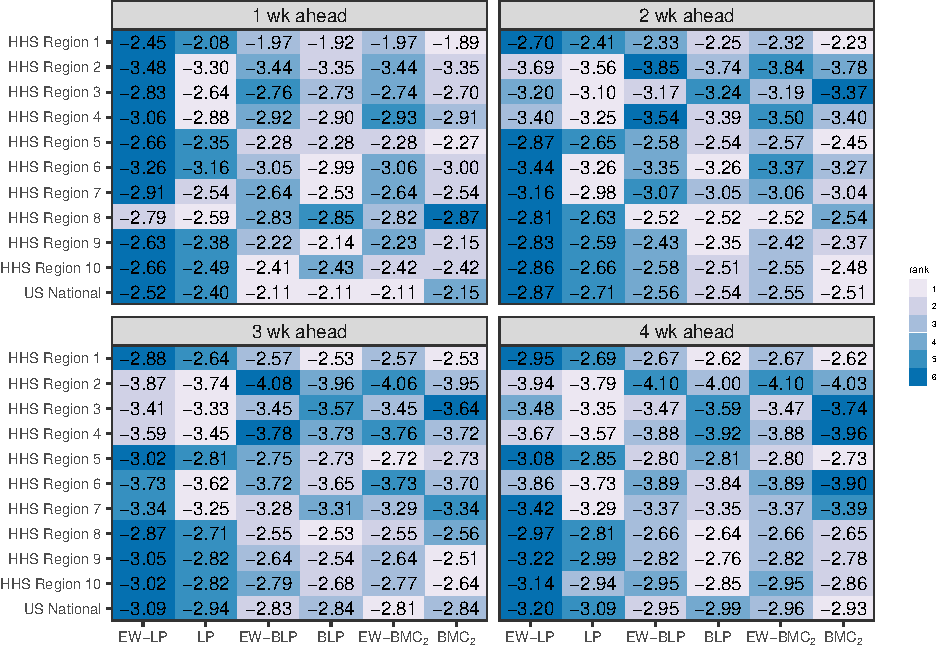
\includegraphics[width=468px]{plot_calibration_files/figure-latex/lsheatloc1-1}

\begin{verbatim}
## pdf 
##   2
\end{verbatim}

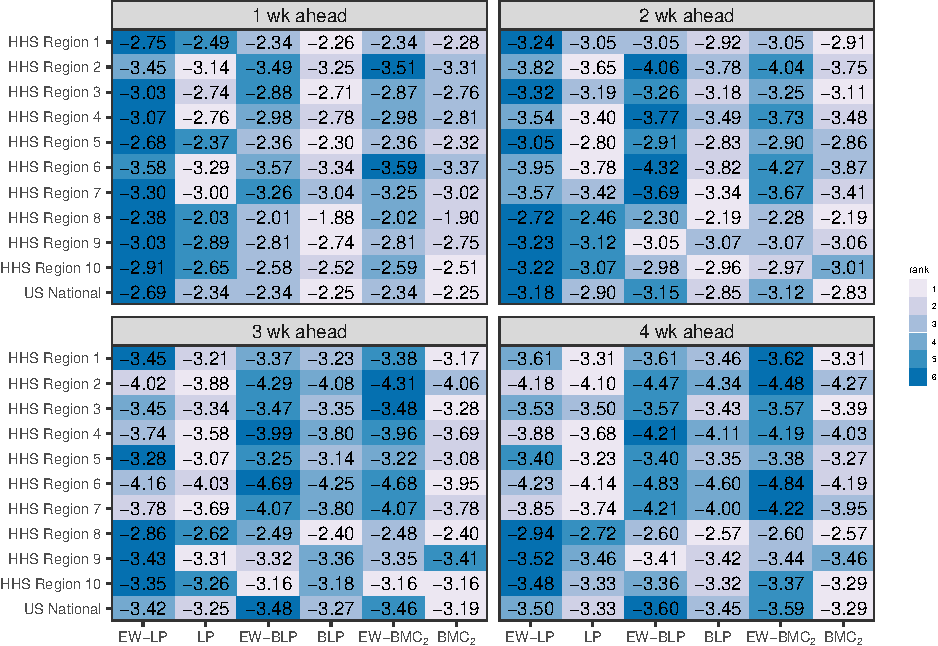
\includegraphics[width=468px]{plot_calibration_files/figure-latex/lsheatloc2-1}

\begin{verbatim}
## pdf 
##   2
\end{verbatim}

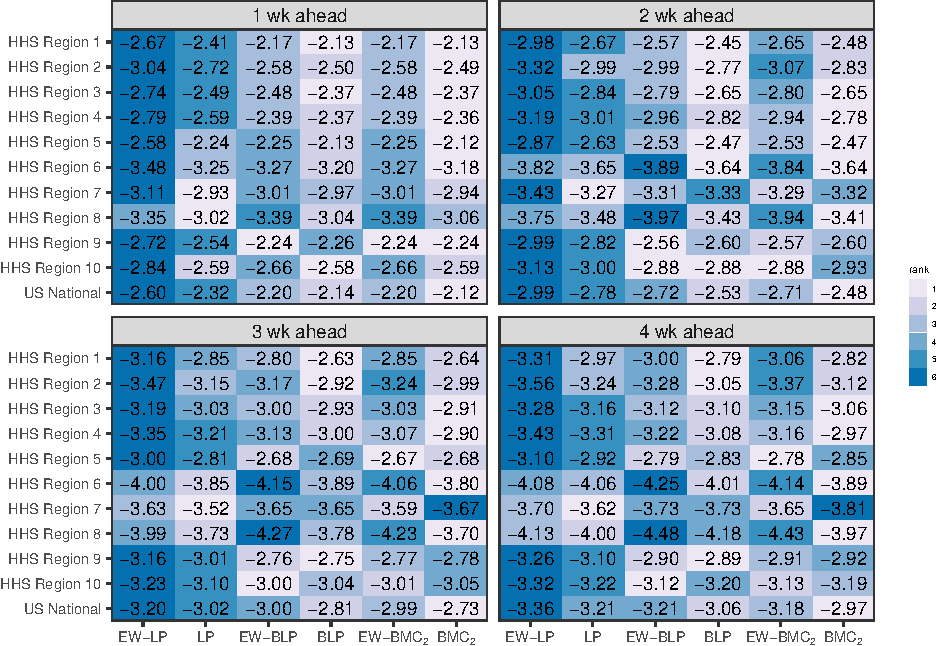
\includegraphics[width=468px]{plot_calibration_files/figure-latex/lsheatloc3-1}

\begin{verbatim}
## pdf 
##   2
\end{verbatim}

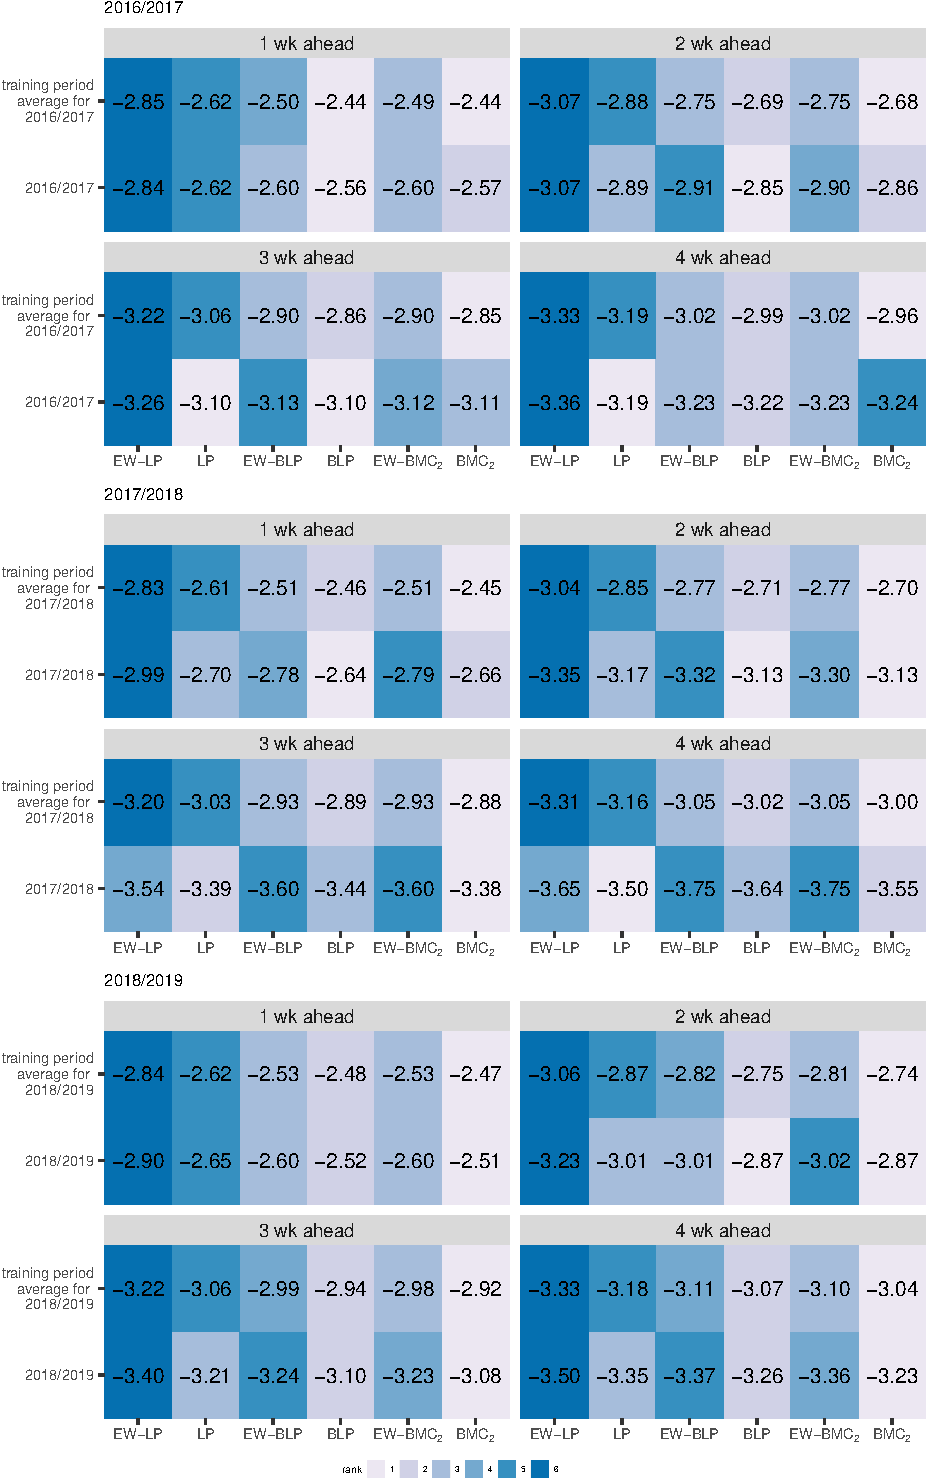
\includegraphics[width=468px]{plot_calibration_files/figure-latex/lsheat1-1}

\begin{verbatim}
## pdf 
##   2
\end{verbatim}

\hypertarget{mean-log-scores-across-all-targets-by-season}{%
\section{Mean log scores across all targets by
season}\label{mean-log-scores-across-all-targets-by-season}}

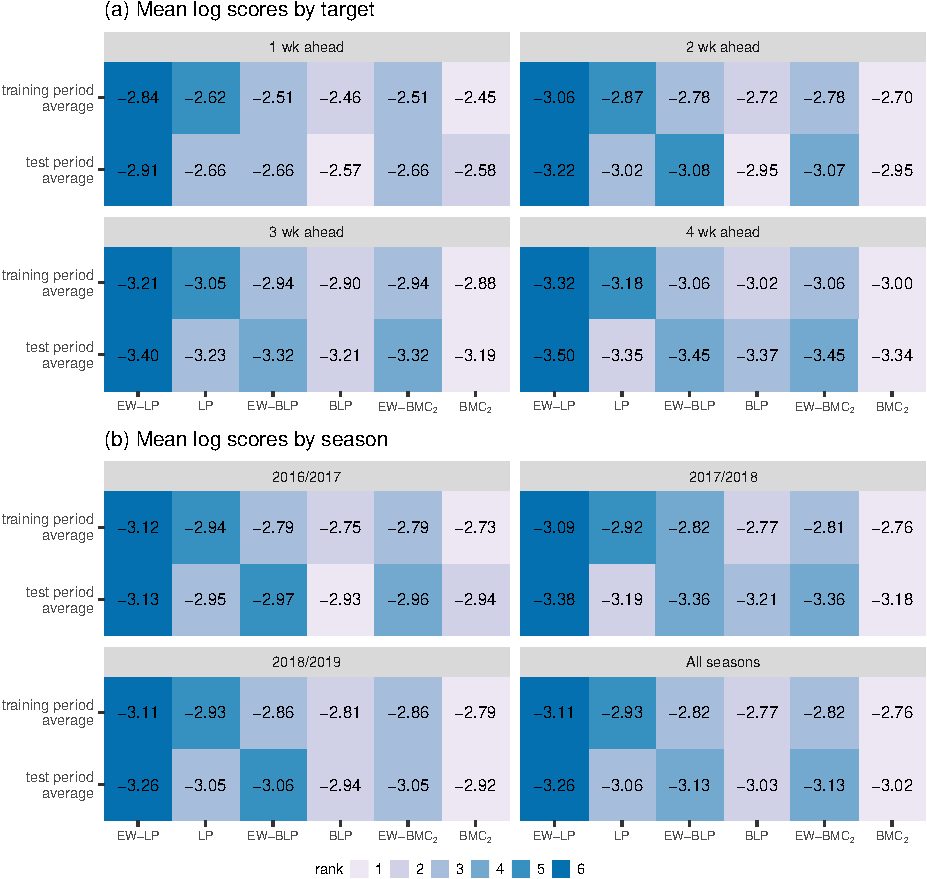
\includegraphics[width=468px]{plot_calibration_files/figure-latex/lsallyear-1}

\hypertarget{box-plot}{%
\section{Box plot}\label{box-plot}}

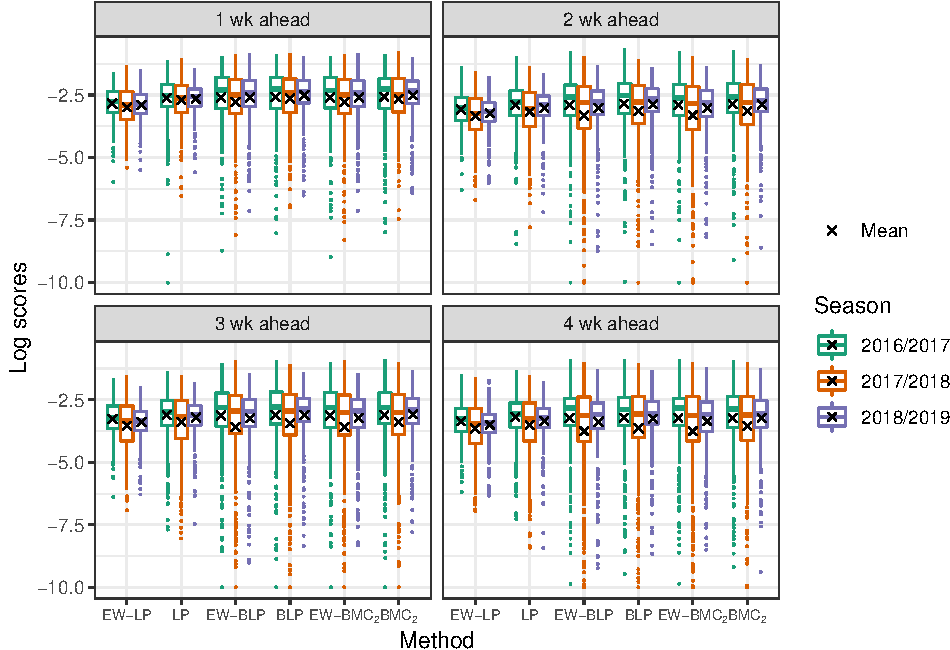
\includegraphics[width=468px]{plot_calibration_files/figure-latex/box-1}

\hypertarget{reliability-plots}{%
\section{Reliability plots}\label{reliability-plots}}

\hypertarget{test-season-20162017}{%
\subsection{Test season 2016/2017}\label{test-season-20162017}}

\begin{tabular}{l|l|r|l}
\hline
target & Method & cd & Season\\
\hline
1 wk ahead & BLP & 0.0048711 & 2016/2017\\
\hline
1 wk ahead & BMC[2] & 0.0041592 & 2016/2017\\
\hline
1 wk ahead & EW-BLP & 0.0054803 & 2016/2017\\
\hline
1 wk ahead & EW-BMC[2] & 0.0064824 & 2016/2017\\
\hline
2 wk ahead & BLP & 0.0038161 & 2016/2017\\
\hline
2 wk ahead & BMC[2] & 0.0050927 & 2016/2017\\
\hline
2 wk ahead & EW-BLP & 0.0051841 & 2016/2017\\
\hline
2 wk ahead & EW-BMC[2] & 0.0066971 & 2016/2017\\
\hline
3 wk ahead & BLP & 0.0041341 & 2016/2017\\
\hline
3 wk ahead & BMC[2] & 0.0052037 & 2016/2017\\
\hline
3 wk ahead & EW-BLP & 0.0050527 & 2016/2017\\
\hline
3 wk ahead & EW-BMC[2] & 0.0059036 & 2016/2017\\
\hline
4 wk ahead & BLP & 0.0051174 & 2016/2017\\
\hline
4 wk ahead & BMC[2] & 0.0055684 & 2016/2017\\
\hline
4 wk ahead & EW-BLP & 0.0053771 & 2016/2017\\
\hline
4 wk ahead & EW-BMC[2] & 0.0056566 & 2016/2017\\
\hline
1 wk ahead & EW-LP & 0.0149024 & 2016/2017\\
\hline
1 wk ahead & LP & 0.0076165 & 2016/2017\\
\hline
2 wk ahead & EW-LP & 0.0108869 & 2016/2017\\
\hline
2 wk ahead & LP & 0.0043100 & 2016/2017\\
\hline
3 wk ahead & EW-LP & 0.0104716 & 2016/2017\\
\hline
3 wk ahead & LP & 0.0053328 & 2016/2017\\
\hline
4 wk ahead & EW-LP & 0.0099795 & 2016/2017\\
\hline
4 wk ahead & LP & 0.0052039 & 2016/2017\\
\hline
\end{tabular}

\begin{tabular}{l|l|r|l}
\hline
target & Method & cd & Season\\
\hline
1 wk ahead & BLP & 0.0054127 & 2016/2017\\
\hline
1 wk ahead & BMC[2] & 0.0065897 & 2016/2017\\
\hline
1 wk ahead & EW-BLP & 0.0070415 & 2016/2017\\
\hline
1 wk ahead & EW-BMC[2] & 0.0075762 & 2016/2017\\
\hline
2 wk ahead & BLP & 0.0076139 & 2016/2017\\
\hline
2 wk ahead & BMC[2] & 0.0045887 & 2016/2017\\
\hline
2 wk ahead & EW-BLP & 0.0074174 & 2016/2017\\
\hline
2 wk ahead & EW-BMC[2] & 0.0125258 & 2016/2017\\
\hline
3 wk ahead & BLP & 0.0050056 & 2016/2017\\
\hline
3 wk ahead & BMC[2] & 0.0048189 & 2016/2017\\
\hline
3 wk ahead & EW-BLP & 0.0093749 & 2016/2017\\
\hline
3 wk ahead & EW-BMC[2] & 0.0116302 & 2016/2017\\
\hline
4 wk ahead & BLP & 0.0066007 & 2016/2017\\
\hline
4 wk ahead & BMC[2] & 0.0044649 & 2016/2017\\
\hline
4 wk ahead & EW-BLP & 0.0102779 & 2016/2017\\
\hline
4 wk ahead & EW-BMC[2] & 0.0094799 & 2016/2017\\
\hline
1 wk ahead & EW-LP & 0.0131806 & 2016/2017\\
\hline
1 wk ahead & LP & 0.0056276 & 2016/2017\\
\hline
2 wk ahead & EW-LP & 0.0082204 & 2016/2017\\
\hline
2 wk ahead & LP & 0.0023943 & 2016/2017\\
\hline
3 wk ahead & EW-LP & 0.0074197 & 2016/2017\\
\hline
3 wk ahead & LP & 0.0030728 & 2016/2017\\
\hline
4 wk ahead & EW-LP & 0.0067265 & 2016/2017\\
\hline
4 wk ahead & LP & 0.0031187 & 2016/2017\\
\hline
\end{tabular}

\begin{itemize}
\item 1 wk ahead: There is evidence of bias in the PIT histograms in both the training and test seasons. The BLP, which outperforms other methods, has a more uniform PIT histogram in the test season.
\item 1 wk ahead: The training PIT histograms for BMC2, EW-BLP, and EW-BMC2 look more uniform compared to that of BLP, maybe overfitting?
\item 2 Week Ahead: There is evidence of some bias in the PIT histograms in both the training and test seasons but less than the previous target. The BLP, which outperforms other methods, has a more uniform PIT histogram in the test season.
\item 3 Week Ahead: There is evidence of some bias in the PIT histograms in both the training and test seasons. The BLP, which outperforms other methods, has a more uniform PIT histogram in the test season.
\item 3 Week Ahead: There might be some overfitting going on, the train PIT histograms look a lot better than the test PIT histograms.
\item 4 Week Ahead: There is evidence of a little bias in the PIT histograms in both the training and test seasons. 
\item 4 Week Ahead: The BLP, EW-BLP, BMC2, and EW-BMC2 are relatively well-calibrated in the training seasons which outperforms other methods, has a more uniform PIT histogram in the test season.
\item 4 Week Ahead: LP outperforms other methods in terms of mean test log score, but the beta methods seem to have more uniform PIT histograms.
\end{itemize}

\newpage

\newpage

\hypertarget{test-season-20172018}{%
\subsection{Test season 2017/2018}\label{test-season-20172018}}

\begin{tabular}{l|l|r|l}
\hline
target & Method & cd & Season\\
\hline
1 wk ahead & BLP & 0.0052980 & 2017/2018\\
\hline
1 wk ahead & BMC[2] & 0.0052071 & 2017/2018\\
\hline
1 wk ahead & EW-BLP & 0.0057044 & 2017/2018\\
\hline
1 wk ahead & EW-BMC[2] & 0.0049287 & 2017/2018\\
\hline
2 wk ahead & BLP & 0.0037963 & 2017/2018\\
\hline
2 wk ahead & BMC[2] & 0.0050105 & 2017/2018\\
\hline
2 wk ahead & EW-BLP & 0.0051559 & 2017/2018\\
\hline
2 wk ahead & EW-BMC[2] & 0.0054119 & 2017/2018\\
\hline
3 wk ahead & BLP & 0.0037003 & 2017/2018\\
\hline
3 wk ahead & BMC[2] & 0.0044498 & 2017/2018\\
\hline
3 wk ahead & EW-BLP & 0.0055969 & 2017/2018\\
\hline
3 wk ahead & EW-BMC[2] & 0.0064533 & 2017/2018\\
\hline
4 wk ahead & BLP & 0.0046367 & 2017/2018\\
\hline
4 wk ahead & BMC[2] & 0.0048347 & 2017/2018\\
\hline
4 wk ahead & EW-BLP & 0.0058855 & 2017/2018\\
\hline
4 wk ahead & EW-BMC[2] & 0.0057387 & 2017/2018\\
\hline
1 wk ahead & EW-LP & 0.0146048 & 2017/2018\\
\hline
1 wk ahead & LP & 0.0076294 & 2017/2018\\
\hline
2 wk ahead & EW-LP & 0.0111236 & 2017/2018\\
\hline
2 wk ahead & LP & 0.0038998 & 2017/2018\\
\hline
3 wk ahead & EW-LP & 0.0103352 & 2017/2018\\
\hline
3 wk ahead & LP & 0.0047050 & 2017/2018\\
\hline
4 wk ahead & EW-LP & 0.0103869 & 2017/2018\\
\hline
4 wk ahead & LP & 0.0047774 & 2017/2018\\
\hline
\end{tabular}

\begin{tabular}{l|l|r|l}
\hline
target & Method & cd & Season\\
\hline
1 wk ahead & BLP & 0.0079406 & 2017/2018\\
\hline
1 wk ahead & BMC[2] & 0.0104345 & 2017/2018\\
\hline
1 wk ahead & EW-BLP & 0.0120691 & 2017/2018\\
\hline
1 wk ahead & EW-BMC[2] & 0.0113115 & 2017/2018\\
\hline
2 wk ahead & BLP & 0.0222152 & 2017/2018\\
\hline
2 wk ahead & BMC[2] & 0.0258332 & 2017/2018\\
\hline
2 wk ahead & EW-BLP & 0.0320468 & 2017/2018\\
\hline
2 wk ahead & EW-BMC[2] & 0.0377415 & 2017/2018\\
\hline
3 wk ahead & BLP & 0.0275273 & 2017/2018\\
\hline
3 wk ahead & BMC[2] & 0.0265708 & 2017/2018\\
\hline
3 wk ahead & EW-BLP & 0.0339585 & 2017/2018\\
\hline
3 wk ahead & EW-BMC[2] & 0.0372751 & 2017/2018\\
\hline
4 wk ahead & BLP & 0.0356719 & 2017/2018\\
\hline
4 wk ahead & BMC[2] & 0.0305636 & 2017/2018\\
\hline
4 wk ahead & EW-BLP & 0.0399702 & 2017/2018\\
\hline
4 wk ahead & EW-BMC[2] & 0.0441642 & 2017/2018\\
\hline
1 wk ahead & EW-LP & 0.0146305 & 2017/2018\\
\hline
1 wk ahead & LP & 0.0072097 & 2017/2018\\
\hline
2 wk ahead & EW-LP & 0.0155284 & 2017/2018\\
\hline
2 wk ahead & LP & 0.0101059 & 2017/2018\\
\hline
3 wk ahead & EW-LP & 0.0151232 & 2017/2018\\
\hline
3 wk ahead & LP & 0.0102632 & 2017/2018\\
\hline
4 wk ahead & EW-LP & 0.0189182 & 2017/2018\\
\hline
4 wk ahead & LP & 0.0122629 & 2017/2018\\
\hline
\end{tabular}

\begin{itemize}
\item 1 Week Ahead There is evidence of some bias in the PIT histograms in both the training and test seasons. The BLP, which outperforms other methods, has a more uniform PIT histogram in the test season, but it is not very calibrated.
\item 2 Week Ahead: There is evidence of some bias in the PIT histograms in both the training and test seasons. Overall the PIT histograms for the beta methods do not look uniform for the test season, despite being relatively well calibrated for the training seasons
\item 2 Week Ahead: The BLP, which outperforms other methods, does not seem to be more calibrated than the LP in the test season.
\item 3 Week Ahead: We have a similar situation here as in the previous target of the same year, but the tail calibration is much worse.
\item 3 Week Ahead: BMC2 is the best performing method in terms of mean log score, but again it does not seem more calibrated than LP (or worse even).
\item 4 Week Ahead: PIT histograms for the training season look well calibrated, but very uncalibrated for the test seasons.
\item 4 Week Ahead: LP outperforms other methods here in terms of log score, and the PIT histograms agree.
\item 4 Week Ahead: For this season, it is possible the poor calibration is a result from training seasons being very different from the test season (bad flu season in 2017/2018), so we have a lot of overfitting. This phenomenon is more apparent for 3-4 week ahead targets.
\end{itemize}

\newpage

\hypertarget{test-season-20182019}{%
\subsection{Test season 2018/2019}\label{test-season-20182019}}

\begin{tabular}{l|l|r|l}
\hline
target & Method & cd & Season\\
\hline
1 wk ahead & BLP & 0.0044834 & 2018/2019\\
\hline
1 wk ahead & BMC[2] & 0.0054616 & 2018/2019\\
\hline
1 wk ahead & EW-BLP & 0.0062674 & 2018/2019\\
\hline
1 wk ahead & EW-BMC[2] & 0.0063125 & 2018/2019\\
\hline
2 wk ahead & BLP & 0.0052216 & 2018/2019\\
\hline
2 wk ahead & BMC[2] & 0.0061713 & 2018/2019\\
\hline
2 wk ahead & EW-BLP & 0.0061392 & 2018/2019\\
\hline
2 wk ahead & EW-BMC[2] & 0.0082081 & 2018/2019\\
\hline
3 wk ahead & BLP & 0.0051157 & 2018/2019\\
\hline
3 wk ahead & BMC[2] & 0.0064120 & 2018/2019\\
\hline
3 wk ahead & EW-BLP & 0.0068349 & 2018/2019\\
\hline
3 wk ahead & EW-BMC[2] & 0.0073993 & 2018/2019\\
\hline
4 wk ahead & BLP & 0.0052746 & 2018/2019\\
\hline
4 wk ahead & BMC[2] & 0.0067850 & 2018/2019\\
\hline
4 wk ahead & EW-BLP & 0.0066245 & 2018/2019\\
\hline
4 wk ahead & EW-BMC[2] & 0.0078157 & 2018/2019\\
\hline
1 wk ahead & EW-LP & 0.0150184 & 2018/2019\\
\hline
1 wk ahead & LP & 0.0081770 & 2018/2019\\
\hline
2 wk ahead & EW-LP & 0.0104274 & 2018/2019\\
\hline
2 wk ahead & LP & 0.0035050 & 2018/2019\\
\hline
3 wk ahead & EW-LP & 0.0099872 & 2018/2019\\
\hline
3 wk ahead & LP & 0.0046804 & 2018/2019\\
\hline
4 wk ahead & EW-LP & 0.0097884 & 2018/2019\\
\hline
4 wk ahead & LP & 0.0044743 & 2018/2019\\
\hline
\end{tabular}

\begin{tabular}{l|l|r|l}
\hline
target & Method & cd & Season\\
\hline
1 wk ahead & BLP & 0.0047974 & 2018/2019\\
\hline
1 wk ahead & BMC[2] & 0.0026731 & 2018/2019\\
\hline
1 wk ahead & EW-BLP & 0.0039126 & 2018/2019\\
\hline
1 wk ahead & EW-BMC[2] & 0.0058970 & 2018/2019\\
\hline
2 wk ahead & BLP & 0.0085924 & 2018/2019\\
\hline
2 wk ahead & BMC[2] & 0.0158859 & 2018/2019\\
\hline
2 wk ahead & EW-BLP & 0.0208561 & 2018/2019\\
\hline
2 wk ahead & EW-BMC[2] & 0.0282232 & 2018/2019\\
\hline
3 wk ahead & BLP & 0.0132635 & 2018/2019\\
\hline
3 wk ahead & BMC[2] & 0.0132836 & 2018/2019\\
\hline
3 wk ahead & EW-BLP & 0.0248644 & 2018/2019\\
\hline
3 wk ahead & EW-BMC[2] & 0.0257321 & 2018/2019\\
\hline
4 wk ahead & BLP & 0.0162236 & 2018/2019\\
\hline
4 wk ahead & BMC[2] & 0.0177277 & 2018/2019\\
\hline
4 wk ahead & EW-BLP & 0.0303535 & 2018/2019\\
\hline
4 wk ahead & EW-BMC[2] & 0.0309859 & 2018/2019\\
\hline
1 wk ahead & EW-LP & 0.0156431 & 2018/2019\\
\hline
1 wk ahead & LP & 0.0082008 & 2018/2019\\
\hline
2 wk ahead & EW-LP & 0.0176694 & 2018/2019\\
\hline
2 wk ahead & LP & 0.0073131 & 2018/2019\\
\hline
3 wk ahead & EW-LP & 0.0165785 & 2018/2019\\
\hline
3 wk ahead & LP & 0.0105017 & 2018/2019\\
\hline
4 wk ahead & EW-LP & 0.0192520 & 2018/2019\\
\hline
4 wk ahead & LP & 0.0104010 & 2018/2019\\
\hline
\end{tabular}

\begin{center}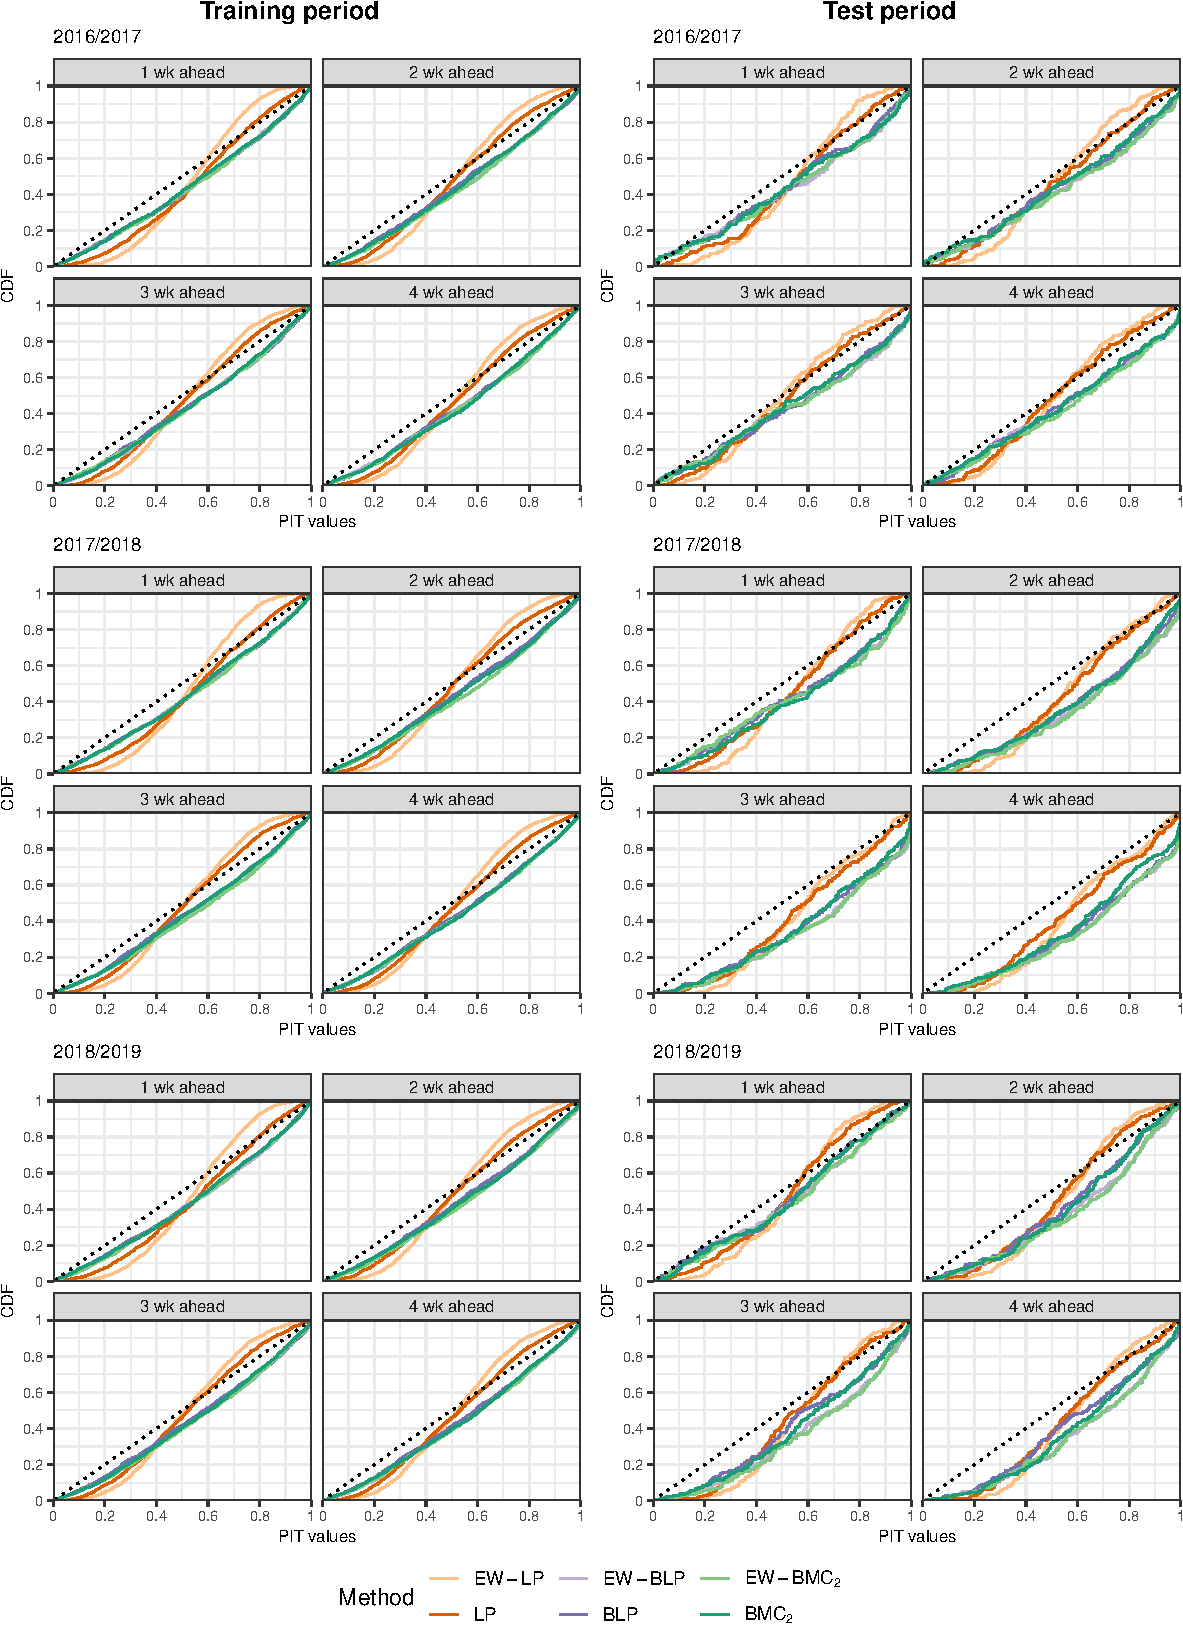
\includegraphics[width=576px]{plot_calibration_files/figure-latex/reli_sup_all-1} \end{center}

\begin{verbatim}
## pdf 
##   2
\end{verbatim}

\begin{itemize}
\item 1 Week Ahead: There is evidence of some bias in the PIT histograms in the training seasons, but look more calibrated for the test season.
\item 1 Week Ahead: The BMC2, which outperforms other methods, does not seem to have a more uniform PIT histogram in the test season compared to other beta methods.
\item 2 Week Ahead: The PIT histograms in the training and test seasons look similar for the beta methods. The BLP, which outperforms other methods, has a more uniform PIT histogram in the test season.
\item 2 Week Ahead: There is evidence of bias.
\item 3 Week Ahead: There is evidence of some bias in the PIT histograms in the test season, but look more calibrated for the training seasons (no surprise here).
\item 3 Week Ahead: The BMC2, which outperforms other methods, does not seem to have a more uniform PIT histogram in the test season compared to other beta methods.
\item 4 Week Ahead: We see a lot bias in the PIT histograms in test seasons, especially for the equally-weighted beta methods, despite the PIT histograms looking well-calibrated for the training seasons.
\item 4 Week Ahead: The BMC2, which outperforms other methods, has a more uniform PIT histogram in the test season compared to other methods. However, these don't look well-calibrated overall.
\end{itemize}

\hypertarget{all-seasons-by-target}{%
\subsection{All seasons by target}\label{all-seasons-by-target}}

\begin{tabular}{l|l|r}
\hline
target & Method & cd\\
\hline
1 wk ahead & BLP & 0.0042051\\
\hline
1 wk ahead & BMC[2] & 0.0046641\\
\hline
1 wk ahead & EW-BLP & 0.0059966\\
\hline
1 wk ahead & EW-BMC[2] & 0.0033702\\
\hline
2 wk ahead & BLP & 0.0024595\\
\hline
2 wk ahead & BMC[2] & 0.0034368\\
\hline
2 wk ahead & EW-BLP & 0.0028310\\
\hline
2 wk ahead & EW-BMC[2] & 0.0030250\\
\hline
3 wk ahead & BLP & 0.0013170\\
\hline
3 wk ahead & BMC[2] & 0.0024463\\
\hline
3 wk ahead & EW-BLP & 0.0022955\\
\hline
3 wk ahead & EW-BMC[2] & 0.0030285\\
\hline
4 wk ahead & BLP & 0.0022758\\
\hline
4 wk ahead & BMC[2] & 0.0021371\\
\hline
4 wk ahead & EW-BLP & 0.0018119\\
\hline
4 wk ahead & EW-BMC[2] & 0.0017686\\
\hline
1 wk ahead & EW-LP & 0.0167291\\
\hline
1 wk ahead & LP & 0.0095898\\
\hline
2 wk ahead & EW-LP & 0.0104907\\
\hline
2 wk ahead & LP & 0.0034801\\
\hline
3 wk ahead & EW-LP & 0.0107914\\
\hline
3 wk ahead & LP & 0.0042957\\
\hline
4 wk ahead & EW-LP & 0.0093535\\
\hline
4 wk ahead & LP & 0.0037497\\
\hline
\end{tabular}

\begin{tabular}{l|l|r}
\hline
target & Method & cd\\
\hline
1 wk ahead & BLP & 0.0028153\\
\hline
1 wk ahead & BMC[2] & 0.0033716\\
\hline
1 wk ahead & EW-BLP & 0.0087785\\
\hline
1 wk ahead & EW-BMC[2] & 0.0039680\\
\hline
2 wk ahead & BLP & 0.0081414\\
\hline
2 wk ahead & BMC[2] & 0.0137705\\
\hline
2 wk ahead & EW-BLP & 0.0168545\\
\hline
2 wk ahead & EW-BMC[2] & 0.0189500\\
\hline
3 wk ahead & BLP & 0.0100588\\
\hline
3 wk ahead & BMC[2] & 0.0128707\\
\hline
3 wk ahead & EW-BLP & 0.0161954\\
\hline
3 wk ahead & EW-BMC[2] & 0.0179540\\
\hline
4 wk ahead & BLP & 0.0123582\\
\hline
4 wk ahead & BMC[2] & 0.0141891\\
\hline
4 wk ahead & EW-BLP & 0.0186291\\
\hline
4 wk ahead & EW-BMC[2] & 0.0206465\\
\hline
1 wk ahead & EW-LP & 0.0131186\\
\hline
1 wk ahead & LP & 0.0066935\\
\hline
2 wk ahead & EW-LP & 0.0099048\\
\hline
2 wk ahead & LP & 0.0041623\\
\hline
3 wk ahead & EW-LP & 0.0098447\\
\hline
3 wk ahead & LP & 0.0047418\\
\hline
4 wk ahead & EW-LP & 0.0087522\\
\hline
4 wk ahead & LP & 0.0048842\\
\hline
\end{tabular}

\begin{center}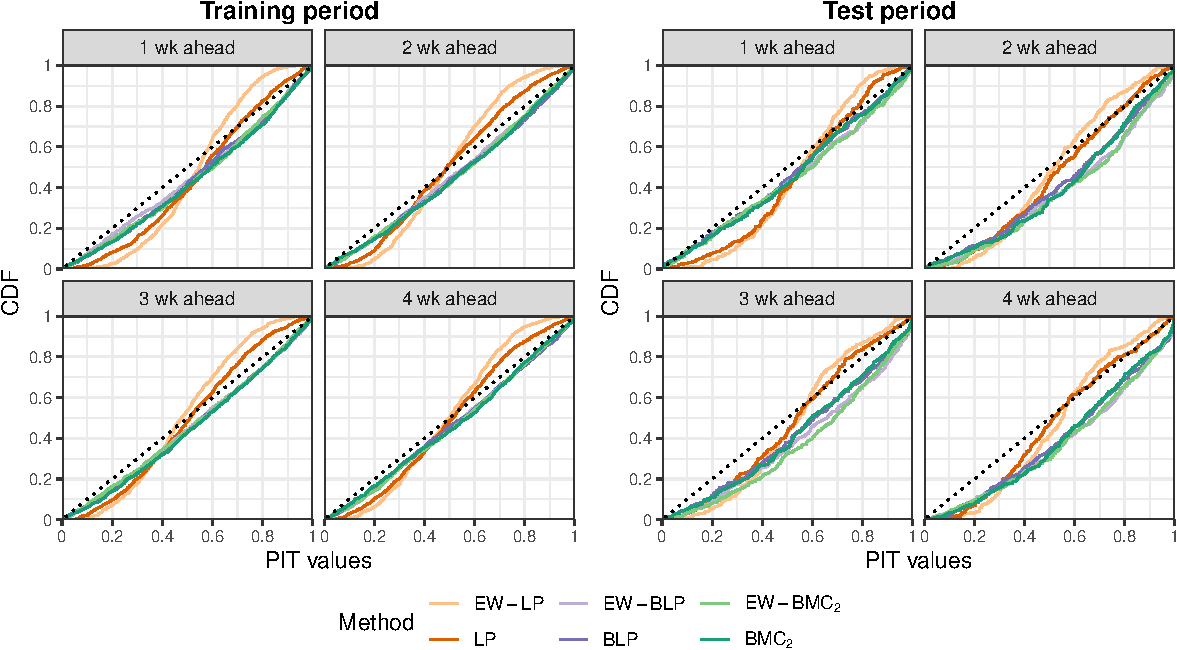
\includegraphics[width=576px]{plot_calibration_files/figure-latex/reli_main-1} \end{center}

\begin{verbatim}
## pdf 
##   2
\end{verbatim}

\begin{center}\includegraphics[width=648px]{plot_calibration_files/figure-latex/reli5-1} \end{center}

\begin{center}\includegraphics[width=576px]{plot_calibration_files/figure-latex/reli6-1} \end{center}
\newpage

\hypertarget{plot-flu-data}{%
\subsection{Plot Flu data}\label{plot-flu-data}}

\begin{verbatim}
## 
## Attaching package: 'lubridate'
\end{verbatim}

\begin{verbatim}
## The following objects are masked from 'package:base':
## 
##     date, intersect, setdiff, union
\end{verbatim}

\begin{center}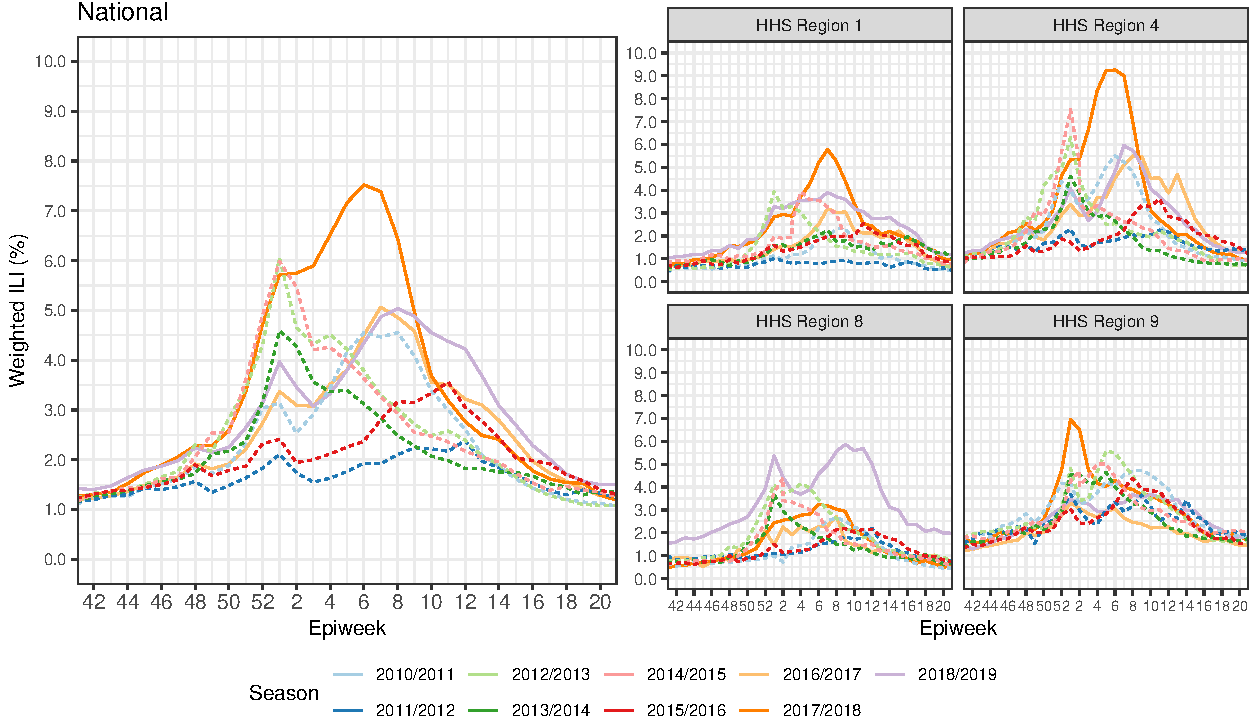
\includegraphics[width=612px]{plot_calibration_files/figure-latex/fludat2-1} \end{center}

\hypertarget{beta-transformation}{%
\subsection{Beta transformation}\label{beta-transformation}}

\begin{verbatim}
## Warning in dnorm(y, mu2, sigma2): NaNs produced
\end{verbatim}

\begin{verbatim}
## Warning in nlm(mixt.deviance, c(0.25, 52, 82, 10, 10), y): NA/Inf replaced by
## maximum positive value
\end{verbatim}

\begin{verbatim}
## Warning in log(pdf): NaNs produced
\end{verbatim}

\begin{verbatim}
## Warning in nlm(mixt.deviance, c(0.25, 52, 82, 10, 10), y): NA/Inf replaced by
## maximum positive value
\end{verbatim}

\begin{verbatim}
## Warning in log(pdf): NaNs produced
\end{verbatim}

\begin{verbatim}
## Warning in nlm(mixt.deviance, c(0.25, 52, 82, 10, 10), y): NA/Inf replaced by
## maximum positive value
\end{verbatim}

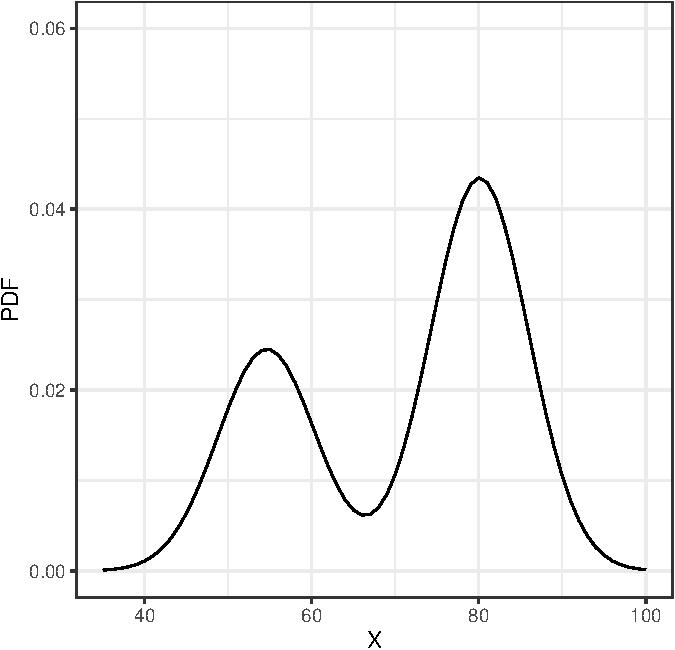
\includegraphics[width=468px]{plot_calibration_files/figure-latex/t1-1}

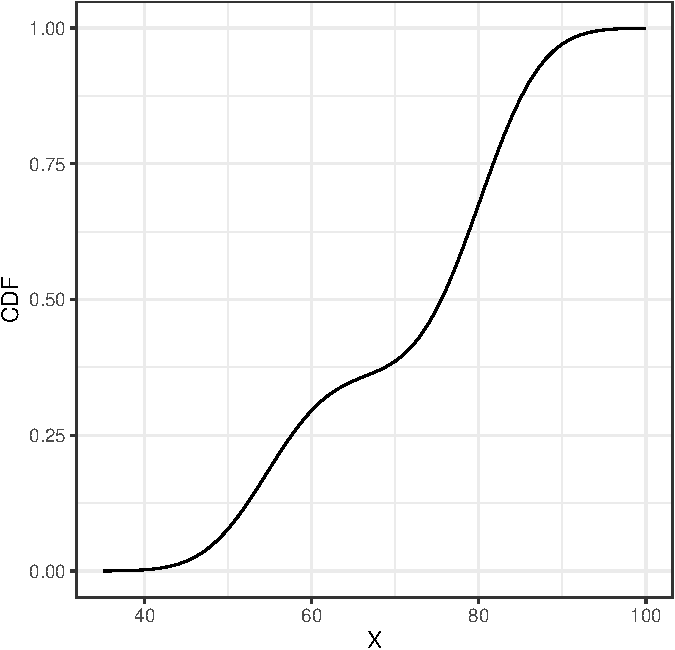
\includegraphics[width=468px]{plot_calibration_files/figure-latex/t2-1}

\begin{verbatim}
## [1] 0.07792616 0.38661624 0.97083274
\end{verbatim}

\begin{verbatim}
## [1] 0.0327599 0.5015517 0.9999029
\end{verbatim}

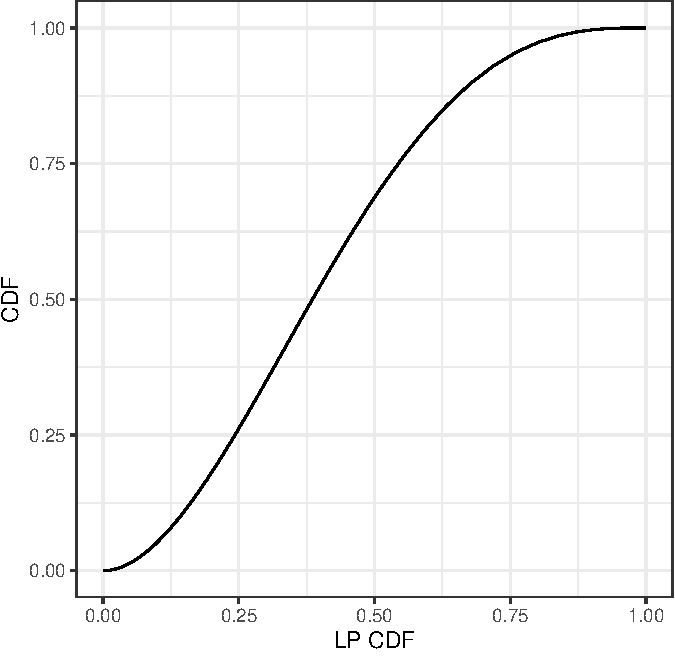
\includegraphics[width=468px]{plot_calibration_files/figure-latex/t3-1}

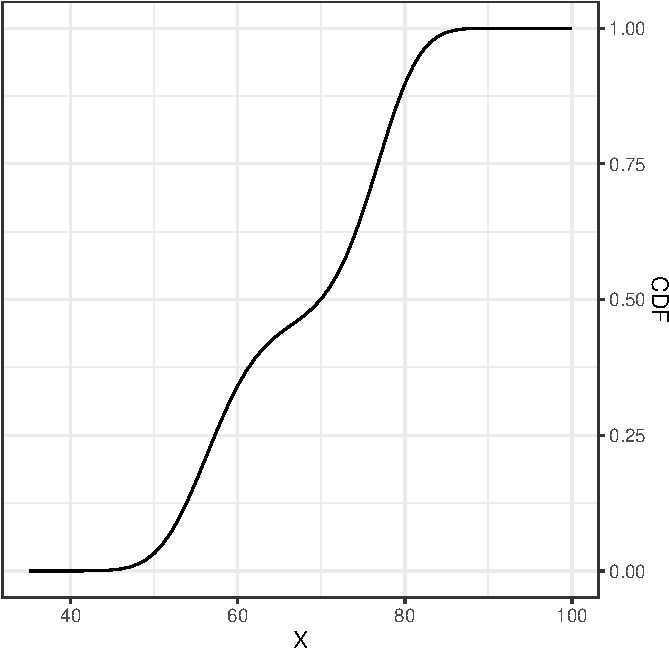
\includegraphics[width=468px]{plot_calibration_files/figure-latex/t4-1}

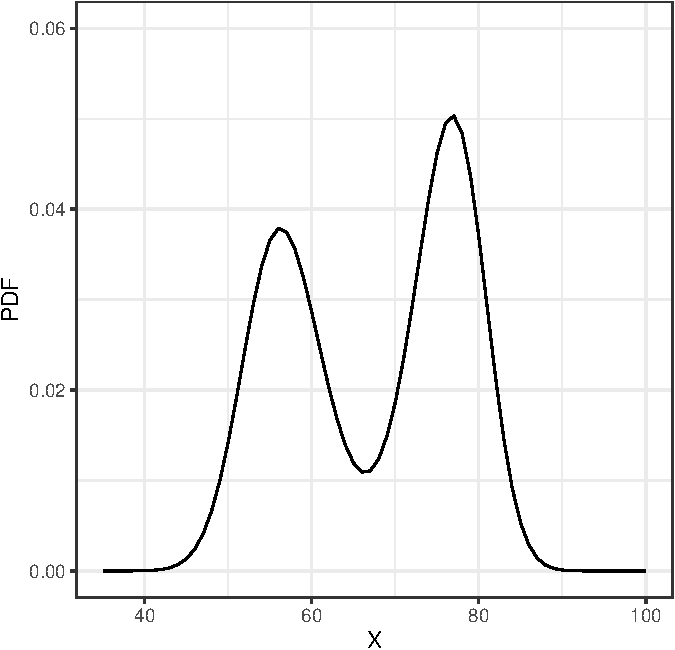
\includegraphics[width=468px]{plot_calibration_files/figure-latex/t5-1}

\end{document}
